% Généré par analysis/analyse.py -- ne pas modifier à la main.
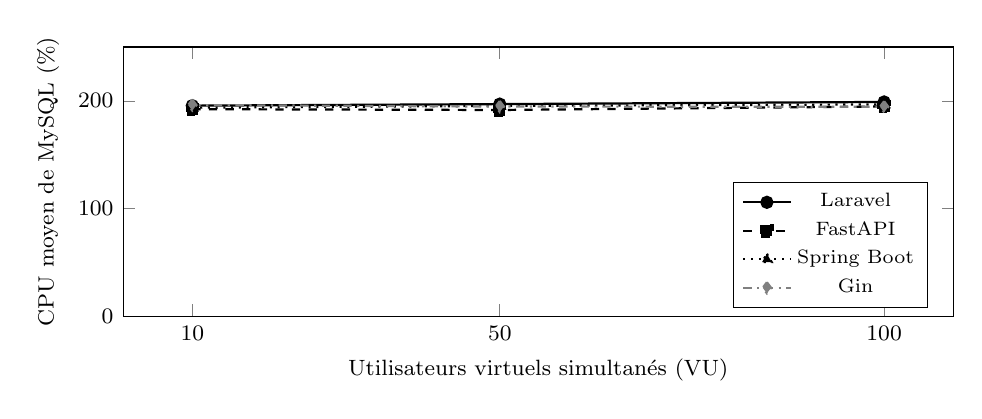
\begin{tikzpicture}
\begin{axis}[
  width=\columnwidth, height=5cm,
  xlabel={Utilisateurs virtuels simultanés (VU)},
  ylabel={CPU moyen de MySQL (\%)},
  xtick={10,50,100},
  tick label style={font=\footnotesize},
  label style={font=\footnotesize},
  legend style={font=\scriptsize, at={(0.97,0.03)}, anchor=south east},
  ymin=0,
  ymax=250]
\addplot[black, thick, mark=*, error bars/.cd, y dir=both, y explicit]
  coordinates {(10,195.53) +- (0,2.07) (50,196.97) +- (0,1.90) (100,198.98) +- (0,1.51)};
\addplot[black, thick, dashed, mark=square*, error bars/.cd, y dir=both, y explicit]
  coordinates {(10,192.26) +- (0,2.47) (50,191.50) +- (0,1.87) (100,194.76) +- (0,2.26)};
\addplot[black, thick, dotted, mark=triangle*, error bars/.cd, y dir=both, y explicit]
  coordinates {(10,193.66) +- (0,1.94) (50,195.29) +- (0,2.02) (100,196.70) +- (0,1.90)};
\addplot[gray, thick, dashdotted, mark=diamond*, error bars/.cd, y dir=both, y explicit]
  coordinates {(10,196.06) +- (0,1.91) (50,194.69) +- (0,2.08) (100,194.49) +- (0,1.92)};
\legend{Laravel, FastAPI, Spring Boot, Gin}
\end{axis}
\end{tikzpicture}
